\documentclass{article}

% Remember to also load the algostyle.sty file into your project.
\usepackage{algostyle}

% Insert new packages here.

\begin{document}
\begin{question}
Recall the $\compproblem{MinVertexCover}$ problem covered in lectures.
\begin{itemize}
    \item[] {\em Given an undirected graph $G = (V, E)$, return the size of the smallest subset $U \subseteq V$ of vertices such that every edge in $E$ is incident to at least one vertex in $U$.}
\end{itemize}

Consider the greedy heuristic: {\em consider the vertex with the largest degree, add that into the vertex cover, and remove the vertex from the graph and all incident edges.}

We will call this algorithm $\compproblem{GreedyVertexCover}$.

\begin{enumerate}[label = (\alph*)]
    \item Exhibit an instance of $G$ that shows that $\compproblem{GreedyVertexCover}$ is suboptimal.

    {\bfseries Note.} {\em You should provide an instance of a graph, what the greedy heuristic would choose, and what a more optimal solution be; the ``more optimal'' solution need not be the most optimal solution, it just needs to beat the greedy solution.}

    We will show that $\compproblem{GreedyVertexCover}$ can be made to perform arbitrarily badly; that is, it is not a constant-approximation algorithm. In particular, we will show that it is an $\Omega(\log n)$-approximation.

    \item We define the bipartite graph $G_n = (L \sqcup R, E)$, where $L$ is a set of $n$ vertices. We define $R$ in parts; for each $2 \leq i \leq n$, let $R_i$ denote a set of $\lfloor n/i \rfloor$ vertices, each with degree $i$. Then $R = R_1 \sqcup R_2 \sqcup \dots \sqcup R_n$. We define the edges such that all vertices of degree $i$ in $L$ are adjacent to distinct vertices in $R$.

    \begin{figure}[H]
        \centering
        \begin{tikzpicture}
            \node[circle, draw, fill = black!10] (a) {};
            \node[circle, draw, fill = black!10, right = 1cm of a] (b) {};
            \node[circle, draw, fill = black!10, right = 1cm of b] (c) {};
            \node[circle, draw, fill = black!10, right = 1cm of c] (d) {};
            \node[circle, draw, fill = black!10, right = 1cm of d] (e) {};
            \node[circle, draw, fill = black!10, right = 1cm of e] (f) {};

            \node[circle, draw = blue, fill = blue!10, below = 2cm of a] (a1) {};
            \node[circle, draw = red, fill = red!10, right = 1cm of a1] (b1) {};
            \node[circle, draw = green!60!black, fill = green!10, right = 1cm of b1] (c1) {};
            \node[circle, draw = purple, fill = purple!10, right = 1cm of c1] (d1) {};
            \node[circle, draw = purple, fill = purple!10, right = 1cm of d1] (d2) {};
            \node[circle, draw = yellow!60!black, fill = yellow!10, right = 1cm of d2] (e1) {};
            \node[circle, draw = yellow!60!black, fill = yellow!10, right = 1cm of e1] (e2) {};
            \node[circle, draw = yellow!60!black, fill = yellow!10, right = 1cm of e2] (e3) {};

            % draw the edges
            \draw[blue] (a1) -- (a);
            \draw[blue] (a1) -- (b);
            \draw[blue] (a1) -- (c);
            \draw[blue] (a1) -- (d);
            \draw[blue] (a1) -- (e);
            \draw[blue] (a1) -- (f);

            \draw[red] (b1) -- (a);
            \draw[red] (b1) -- (b);
            \draw[red] (b1) -- (c);
            \draw[red] (b1) -- (d);
            \draw[red] (b1) -- (e);

            \draw[green!60!black] (c1) -- (a);
            \draw[green!60!black] (c1) -- (b);
            \draw[green!60!black] (c1) -- (c);
            \draw[green!60!black] (c1) -- (d);

            \draw[red!60!black] (d1) -- (a);
            \draw[red!60!black] (d1) -- (b);
            \draw[red!60!black] (d1) -- (c);

            \draw[red!60!black] (d2) -- (d);
            \draw[red!60!black] (d2) -- (e);
            \draw[red!60!black] (d2) -- (f);

            \draw[yellow!60!black] (e1) -- (a);
            \draw[yellow!60!black] (e1) -- (b);
            \draw[yellow!60!black] (e2) -- (c);
            \draw[yellow!60!black] (e2) -- (d);
            \draw[yellow!60!black] (e3) -- (e);
            \draw[yellow!60!black] (e3) -- (f);
        \end{tikzpicture}
        \caption{{\em The graph $G_6$.}}
        \label{fig:enter-label}
    \end{figure}

    What does the greedy algorithm choose? What should the optimal vertex cover be?

    {\bfseries Hint.} {\em Firstly, figure out what the maximum degree of any vertex in $L$ must be and then use the greedy heuristic to decide what vertices the greedy algorithm picks.}

    \item Let $\lvert \compproblem{GreedyVertex} \rvert$ denote the size of the vertex cover chosen by the greedy algorithm, and let $\lvert \compproblem{opt}\rvert$ denote the size of the optimal vertex cover. Prove that \[\lvert \compproblem{GreedyVertex} \rvert \geq n(H_n - 2),\] where $H_n = \sum_{i = 1}^n 1/i$ is the $n$th Harmonic number.
    
    \item Hence, show that $\compproblem{GreedyVertexCover}$ is an $\Omega(\log n)$-approximation by proving that \[\frac{\lvert \compproblem{GreedyVertex} \rvert}{\lvert \compproblem{opt} \rvert} \geq H_n - 2.\]

    {\bfseries Note.} {\em $H_n = \log n + \Theta(1)$; therefore, proving the inequality shows the lower bound approximation.}
\end{enumerate}
\end{question}

\pagebreak

\begin{solution}
\begin{enumerate}[label = (\alph*)]
    \item Example:

    \begin{center}
        
        \tikzset{every picture/.style={line width=0.75pt}} %set default line width to 0.75pt        

        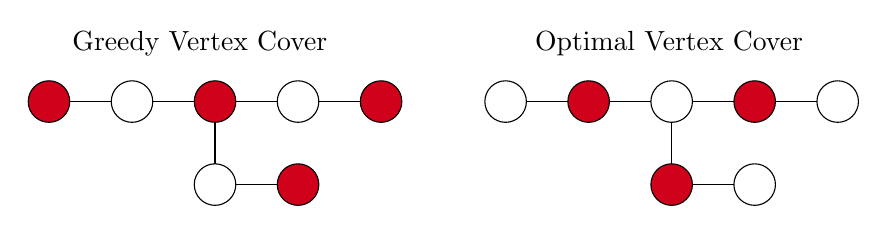
\begin{tikzpicture}[x=0.75pt,y=0.75pt,yscale=-1,xscale=1]
        %uncomment if require: \path (0,300); %set diagram left start at 0, and has height of 300

        %Shape: Ellipse [id:dp9870014619967735] 
        \draw  [fill={rgb, 255:red, 208; green, 2; blue, 27 }  ,fill opacity=1 ] (100.2,130) .. controls (100.2,124.48) and (104.68,120) .. (110.2,120) .. controls (115.72,120) and (120.2,124.48) .. (120.2,130) .. controls (120.2,135.52) and (115.72,140) .. (110.2,140) .. controls (104.68,140) and (100.2,135.52) .. (100.2,130) -- cycle ;
        %Shape: Ellipse [id:dp016180005589067292] 
        \draw   (140.2,130) .. controls (140.2,124.48) and (144.68,120) .. (150.2,120) .. controls (155.72,120) and (160.2,124.48) .. (160.2,130) .. controls (160.2,135.52) and (155.72,140) .. (150.2,140) .. controls (144.68,140) and (140.2,135.52) .. (140.2,130) -- cycle ;
        %Shape: Ellipse [id:dp8722226868836789] 
        \draw  [fill={rgb, 255:red, 208; green, 2; blue, 27 }  ,fill opacity=1 ] (180.2,130) .. controls (180.2,124.48) and (184.68,120) .. (190.2,120) .. controls (195.72,120) and (200.2,124.48) .. (200.2,130) .. controls (200.2,135.52) and (195.72,140) .. (190.2,140) .. controls (184.68,140) and (180.2,135.52) .. (180.2,130) -- cycle ;
        %Shape: Ellipse [id:dp7311768112144386] 
        \draw   (220.2,130) .. controls (220.2,124.48) and (224.68,120) .. (230.2,120) .. controls (235.72,120) and (240.2,124.48) .. (240.2,130) .. controls (240.2,135.52) and (235.72,140) .. (230.2,140) .. controls (224.68,140) and (220.2,135.52) .. (220.2,130) -- cycle ;
        %Shape: Ellipse [id:dp292117241343403] 
        \draw  [fill={rgb, 255:red, 208; green, 2; blue, 27 }  ,fill opacity=1 ] (260.2,130) .. controls (260.2,124.48) and (264.68,120) .. (270.2,120) .. controls (275.72,120) and (280.2,124.48) .. (280.2,130) .. controls (280.2,135.52) and (275.72,140) .. (270.2,140) .. controls (264.68,140) and (260.2,135.52) .. (260.2,130) -- cycle ;
        %Shape: Ellipse [id:dp4544810585968717] 
        \draw   (180.2,170) .. controls (180.2,164.48) and (184.68,160) .. (190.2,160) .. controls (195.72,160) and (200.2,164.48) .. (200.2,170) .. controls (200.2,175.52) and (195.72,180) .. (190.2,180) .. controls (184.68,180) and (180.2,175.52) .. (180.2,170) -- cycle ;
        %Shape: Ellipse [id:dp3899587051902855] 
        \draw  [fill={rgb, 255:red, 208; green, 2; blue, 27 }  ,fill opacity=1 ] (220.2,170) .. controls (220.2,164.48) and (224.68,160) .. (230.2,160) .. controls (235.72,160) and (240.2,164.48) .. (240.2,170) .. controls (240.2,175.52) and (235.72,180) .. (230.2,180) .. controls (224.68,180) and (220.2,175.52) .. (220.2,170) -- cycle ;
        %Straight Lines [id:da010065227226572215] 
        \draw    (120.2,130) -- (140.2,130) ;
        %Straight Lines [id:da7504553995975198] 
        \draw    (160.2,130) -- (180.2,130) ;
        %Straight Lines [id:da9454474417798828] 
        \draw    (200.2,130) -- (220.2,130) ;
        %Straight Lines [id:da6680093477804447] 
        \draw    (240.2,130) -- (260.2,130) ;
        %Straight Lines [id:da36165607288683277] 
        \draw    (190.2,140) -- (190.2,160) ;
        %Straight Lines [id:da3626549296976107] 
        \draw    (220.2,170) -- (200.2,170) ;
        %Shape: Ellipse [id:dp3722092944941977] 
        \draw   (320.2,130) .. controls (320.2,124.48) and (324.68,120) .. (330.2,120) .. controls (335.72,120) and (340.2,124.48) .. (340.2,130) .. controls (340.2,135.52) and (335.72,140) .. (330.2,140) .. controls (324.68,140) and (320.2,135.52) .. (320.2,130) -- cycle ;
        %Shape: Ellipse [id:dp44391271304459745] 
        \draw  [color={rgb, 255:red, 0; green, 0; blue, 0 }  ,draw opacity=1 ][fill={rgb, 255:red, 208; green, 2; blue, 27 }  ,fill opacity=1 ] (360.2,130) .. controls (360.2,124.48) and (364.68,120) .. (370.2,120) .. controls (375.72,120) and (380.2,124.48) .. (380.2,130) .. controls (380.2,135.52) and (375.72,140) .. (370.2,140) .. controls (364.68,140) and (360.2,135.52) .. (360.2,130) -- cycle ;
        %Shape: Ellipse [id:dp8786570793070339] 
        \draw   (400.2,130) .. controls (400.2,124.48) and (404.68,120) .. (410.2,120) .. controls (415.72,120) and (420.2,124.48) .. (420.2,130) .. controls (420.2,135.52) and (415.72,140) .. (410.2,140) .. controls (404.68,140) and (400.2,135.52) .. (400.2,130) -- cycle ;
        %Shape: Ellipse [id:dp14160152778708168] 
        \draw  [fill={rgb, 255:red, 208; green, 2; blue, 27 }  ,fill opacity=1 ] (440.2,130) .. controls (440.2,124.48) and (444.68,120) .. (450.2,120) .. controls (455.72,120) and (460.2,124.48) .. (460.2,130) .. controls (460.2,135.52) and (455.72,140) .. (450.2,140) .. controls (444.68,140) and (440.2,135.52) .. (440.2,130) -- cycle ;
        %Shape: Ellipse [id:dp08525989251871513] 
        \draw   (480.2,130) .. controls (480.2,124.48) and (484.68,120) .. (490.2,120) .. controls (495.72,120) and (500.2,124.48) .. (500.2,130) .. controls (500.2,135.52) and (495.72,140) .. (490.2,140) .. controls (484.68,140) and (480.2,135.52) .. (480.2,130) -- cycle ;
        %Shape: Ellipse [id:dp19296562696810482] 
        \draw  [fill={rgb, 255:red, 208; green, 2; blue, 27 }  ,fill opacity=1 ] (400.2,170) .. controls (400.2,164.48) and (404.68,160) .. (410.2,160) .. controls (415.72,160) and (420.2,164.48) .. (420.2,170) .. controls (420.2,175.52) and (415.72,180) .. (410.2,180) .. controls (404.68,180) and (400.2,175.52) .. (400.2,170) -- cycle ;
        %Shape: Ellipse [id:dp7968549650597094] 
        \draw   (440.2,170) .. controls (440.2,164.48) and (444.68,160) .. (450.2,160) .. controls (455.72,160) and (460.2,164.48) .. (460.2,170) .. controls (460.2,175.52) and (455.72,180) .. (450.2,180) .. controls (444.68,180) and (440.2,175.52) .. (440.2,170) -- cycle ;
        %Straight Lines [id:da4942440409761819] 
        \draw    (340.2,130) -- (360.2,130) ;
        %Straight Lines [id:da610218544169542] 
        \draw    (380.2,130) -- (400.2,130) ;
        %Straight Lines [id:da09524178263425975] 
        \draw    (420.2,130) -- (440.2,130) ;
        %Straight Lines [id:da8040249689990808] 
        \draw    (460.2,130) -- (480.2,130) ;
        %Straight Lines [id:da8363940732830424] 
        \draw    (410.2,140) -- (410.2,160) ;
        %Straight Lines [id:da6122449075144252] 
        \draw    (440.2,170) -- (420.2,170) ;

        % Text Node
        \draw (120.2,94.67) node [anchor=north west][inner sep=0.75pt]   [align=left] {Greedy Vertex Cover};
        % Text Node
        \draw (343.2,94.67) node [anchor=north west][inner sep=0.75pt]   [align=left] {Optimal Vertex Cover};


        \end{tikzpicture}

    \end{center}
    

    \item Each vertex in $L$ is adjacent to at most one vertex in each of $R_2, R_3, \dots , R_n$.
    Therefore the degree of any vertex in $L$ is at most $n - 1$. 
    Therefore the greedy algorithm first picks the vertex in $R_n$.
    The removal of this vertex and all its adjacent edges results in 
    each vertex in $L$ being adjacent to at most one vertex in each of $R_2, R_3, \dots , R_{n-1}$,
    each one therefore having a degree of at most $n - 2$.
    At this point the greedy algorithm would start picking vertices in $R_{n-1}$ as they all have a degree of $n - 1$.
    This results in each vertex in $L$ being adjacent to at most one vertex in each of $R_2, R_3, \dots, R_{n-2}$.
    This process continues until every vertex in $R$ has been selected, where there will be no edges left.

    \item |Greedy Vertex| is equal to the size of $R$.

    \begin{align*}
        |R|&= \left\lfloor \frac{n}{2} \right\rfloor + \left\lfloor \frac{n}{3} \right\rfloor +\dots + \left\lfloor \frac{n}{n} \right\rfloor\\
        &\geq \frac{n}{2} - 1 + \frac{n}{3} - 1 + \dots + \frac{n}{n} - 1\\
        &\geq \frac{n}{1} + \frac{n}{2} + \frac{n}{3} + \frac{n}{n} - \frac{n}{1} - n\\
        &\geq n(H_n - 2)
    \end{align*}
    
    \item Selecting all vertices in $L$ will also give a vertex cover. The size of this vertex cover is $n$.
    Therefore $\lvert \compproblem{Opt} \rvert \leq n$.
    
    \begin{align*}
        \frac{\lvert \compproblem{GreedyVertex} \rvert}{\lvert \compproblem{opt} \rvert} &\geq \frac{\lvert \compproblem{GreedyVertex} \rvert}{n}\\
        &\geq H_2 - 2
    \end{align*}
\end{enumerate}
\end{solution}
\end{document}